%%%%%%%%%%%%%%%%%%%%%%%%%%%%%%%%%%%%%%%%%%%%%%%%%%%%%%%%%%%%%%%%%%%%%%%%%%%%%%%%
% Frontiers in Physics manuscript -- revised version (Major Revision)
% Manuscript ID: 1833442
%%%%%%%%%%%%%%%%%%%%%%%%%%%%%%%%%%%%%%%%%%%%%%%%%%%%%%%%%%%%%%%%%%%%%%%%%%%%%%%%

\documentclass[utf8]{FrontiersinHarvard}

\usepackage{url,hyperref,lineno,microtype,subcaption}
\usepackage[onehalfspacing]{setspace}
\usepackage{amsmath,amssymb}
\usepackage{booktabs}
\usepackage{array}

\linenumbers

% Leave a blank line between paragraphs instead of using \\

\def\keyFont{\fontsize{8}{11}\helveticabold }
\def\firstAuthorLast{Wang}
\def\Authors{Liang Wang\,$^{1,*}$}
\def\Address{$^{1}$School of Artificial Intelligence and Automation, Huazhong University of Science and Technology, Wuhan, P.R. China}
\def\corrAuthor{Liang Wang}
\def\corrEmail{wangliang.f@gmail.com}

\begin{document}
\onecolumn
\firstpage{1}

\title[A Hénon-Map Model for Riemann Zeros]{An Area-Preserving Hénon-Map Model for the Riemann Zeros: A Deterministic-Dynamics Approach with Quantum and Dissipative Solvers}

\author[\firstAuthorLast ]{\Authors}
\address{}
\correspondance{}

\extraAuth{}

\maketitle

\begin{abstract}
\section{}
The Hilbert--P\'olya conjecture proposes that the imaginary parts of the nontrivial Riemann zeros are the eigenvalues of a self-adjoint operator. Random matrix theory describes their \emph{local} statistics: after unfolding, the pair correlation matches the Gaussian Unitary Ensemble (GUE), with subleading arithmetic corrections from the Hardy--Littlewood conjectures. Building on our finding that the symbolic dynamics of the Logistic map at its band-merging point is isomorphic to the prime sieve [Wang, \emph{Research in Mathematics} 13(1), 2026], we ask a constructive question: can a single low-dimensional deterministic system reproduce both the global counting function of the zeros and their local repulsion? The one-dimensional Logistic map is dissipative ($\det J\to0$) and cannot host a unitary spectrum, so we lift it to the two-dimensional area-preserving Hénon map ($\det J=1$) and analyze its spectrum near the edge of chaos. From the map's continuum limit we build a quartic-regularized Hamiltonian and two independent eigensolvers --- a unitary Fourier (quantum) solver and a Markovian Fokker--Planck (dissipative) solver --- and compare to the first 100 zeros. With single-point anchoring, the quantum solver reaches a best mean absolute percentage error of $2.3\%$ (a sharp optimum) and a robust $\approx10$--$20\%$ across grids and regularizations; the dissipative solver reaches $6.5\%$. A globally fitted GUE surrogate shows systematic deviation in the same comparison. The quantum solver's Floquet eigenphases show GUE-type level repulsion, though such statistics are generic to chaotic systems; the distinctive result is the agreement with the actual zero values. We present these as numerical observations and heuristic arguments rather than proofs, and state explicitly which claims are conjectural, numerical, or established.

\tiny
\keyFont{ \section{Keywords:} Riemann zeros, H\'enon map, area-preserving dynamics, quantum chaos, Hilbert--P\'olya conjecture, Fokker--Planck dynamics, spectral statistics}
\end{abstract}

\section{Introduction}

\subsection{The Hilbert--P\'olya conjecture and the dynamical viewpoint}

Since Riemann's 1859 memoir \citep{riemann1859} connected the distribution of primes to the nontrivial zeros of the $\zeta$ function, the Riemann Hypothesis --- that all nontrivial zeros $\rho = 1/2 + i\gamma_n$ lie on the critical line --- has remained central to both mathematics and mathematical physics \citep{titchmarsh1986,sarnak2000}. The Hilbert--P\'olya conjecture offers a physical route to this statement: if the ordinates $\gamma_n$ are the eigenvalues of a self-adjoint operator, their reality follows automatically \citep{schumayer2011}. This idea has motivated a long line of candidate operators and quantization schemes, from the Berry--Keating $H = xp$ proposal \citep{berry1999} and its Bender--Brody--M\"uller variant \citep{bender2017}, to the modified-commutator generalizations explored by \citet{bishop2019}, as well as approaches based on noncommutative geometry \citep{connes1999} and Landau levels \citep{sierra2008}. We emphasize at the outset that the present work does \emph{not} claim to identify the Hilbert--P\'olya operator or to prove any statement about the zeros; it explores a specific deterministic dynamical system as a numerical model whose spectrum is compared to the zeros.

\subsection{Random matrix theory: what it does and does not assert}

A foundational result in this area is the agreement between the local statistics of the Riemann zeros and those of the GUE. Montgomery's pair-correlation conjecture \citep{montgomery1973}, together with Dyson's identification of the corresponding random-matrix form \citep{dyson1962} and Odlyzko's high-precision numerical confirmation \citep{odlyzko1987}, established this connection, which sits within the Bohigas--Giannoni--Schmit framework relating quantum chaos to RMT \citep{bohigas1984,gutzwiller1990}.

It is important to state the RMT position accurately, as our earlier draft did not. The GUE correspondence concerns the \emph{unfolded local} spectral statistics: one first removes the smooth, slowly varying mean density $\bar{N}(E)\sim (E/2\pi)\log(E/2\pi)$ \citep{weyl1911} --- which is dictated by the prime number theorem \citep{hadamard1896} --- so that the rescaled spacings have unit mean, and only then compares correlation functions. RMT does \emph{not} assert that a finite Wigner semicircle reproduces the global counting function of the zeros; the unfolding step removes exactly that global information. Moreover, the deviations of the zeros from pure GUE behavior are not failures of RMT but carry arithmetic content: the subleading, non-universal corrections to the pair correlation are equivalent to the Hardy--Littlewood twin-prime conjecture, as shown by \citet{keating2019}. We thank the reviewers for pressing this point.

Given this, our motivation is not to claim that RMT ``fails.'' Rather, we ask a constructive and complementary question: \emph{can a single, low-dimensional deterministic dynamical system generate, within one model and without a manual unfolding step, both the global mean density and the local repulsion of the zeros?} A positive numerical answer would not contradict RMT; it would offer a concrete dynamical object whose spectrum exhibits both scales simultaneously, in the spirit of the Hilbert--P\'olya program.

\subsection{From a published prime--chaos isomorphism to a 2D area-preserving map}

The starting point of this paper is a result we have recently published. In \citet{wang2026} we showed that the symbolic dynamics of the one-dimensional Logistic map at its band-merging point ($u_c \approx 1.5437$) is isomorphic to the symbolic structure of the prime sieve, and that the Hardy--Littlewood twin-prime constant ($C_2 \approx 0.6602$) emerges as a fixed point of that dynamical system to a numerical precision better than $10^{-4}$ without parameter tuning. That work concerns the \emph{primes themselves}; the present work asks the natural follow-up question dictated by the Hilbert--P\'olya viewpoint: if a deterministic map encodes the arithmetic of the sieve, what is the \emph{spectrum} associated with it, and how does that spectrum compare to the Riemann zeros?

The Logistic map is, however, strongly dissipative: its Jacobian determinant collapses ($\det J \to 0$), phase-space volume is not conserved, and the dynamics are not time-reversible. Such a system cannot support the unitary, time-reversal-respecting structure required for a real, Hermitian-like spectrum in the Hilbert--P\'olya sense; a spectrum extracted directly from it would generically drift into the complex plane. This is a structural obstruction, not a numerical one. We therefore lift the dynamics to the two-dimensional area-preserving H\'enon map \citep{henon1969}, in which the area-preserving constraint ($\det J = 1$) restores volume conservation and time-reversal symmetry. The remainder of the paper performs a spectral analysis of this 2D map near the edge of chaos and compares the resulting eigenvalues with the Riemann zeros, using two numerically independent solvers as a cross-check.

\subsection{Scope and claims}

Because the subject touches the Riemann Hypothesis, we are explicit about the epistemic status of our statements. This paper reports (i) a structural argument for moving from a 1D dissipative map to a 2D area-preserving map; (ii) a numerical determination of a critical parameter associated with a homoclinic tangency; (iii) numerical comparisons between the spectra of two independent solvers and the first 100 Riemann zeros; and (iv) a qualitative comparison with published quantum-hardware decoherence data. None of these constitutes a proof that the spectrum of our operator coincides with the zeros, and we do not claim otherwise. Table~\ref{tab:claims} summarizes the status of each claim. We have correspondingly removed the proof-level and promotional language of the previous version.

\section{Materials and Methods}

\subsection{From the 1D dissipative map to the 2D area-preserving map}

A semiclassical heuristic for level repulsion is that the underlying classical dynamics should occupy a mixed phase space in which regular and chaotic regions coexist. As noted above, the 1D Logistic map $x_{n+1} = 1 - u\,x_n^2$ that we used in \citet{wang2026} to model the prime sieve is dissipative: $\det J \to 0$, the maximal Lyapunov exponent at the band-merging point is large ($\lambda \approx 0.34$), and time-reversal symmetry is absent. We regard the 1D map as a reduced (dissipative) description of the arithmetic and not as a candidate spectral host.

To restore the structure required by Hilbert--P\'olya, we use the area-preserving H\'enon family with $b=-1$ ($\det J = 1$):
\begin{equation}
x_{n+1} = 1 - a\,x_n^2 - x_{n-1}.
\label{eq:henon}
\end{equation}
In this conservative setting, phase-space volume is preserved and the dynamics are time-reversible. Numerically, the maximal Lyapunov exponent in the regime of interest drops to a weakly chaotic value ($\lambda \approx 0.11$), which is the kind of weak chaos associated with level repulsion while still allowing long-lived (near-)regular structures.

\subsection{Phase-space scan and the parity statistic at $a \approx 1.02$}

In a conservative system the control parameter $a$ governs the breakup of Kolmogorov--Arnold--Moser (KAM) tori. We performed a Monte Carlo scan over $a$, sampling orbits and recording (i) the orbit survival rate (fraction of initial conditions remaining bounded) and (ii) a symbolic ``LL'' statistic that counts consecutive same-side excursions, the dynamical analogue of the consecutive-odd-cluster prohibition identified in \citet{wang2026}.

\begin{figure}[h!]
\begin{center}
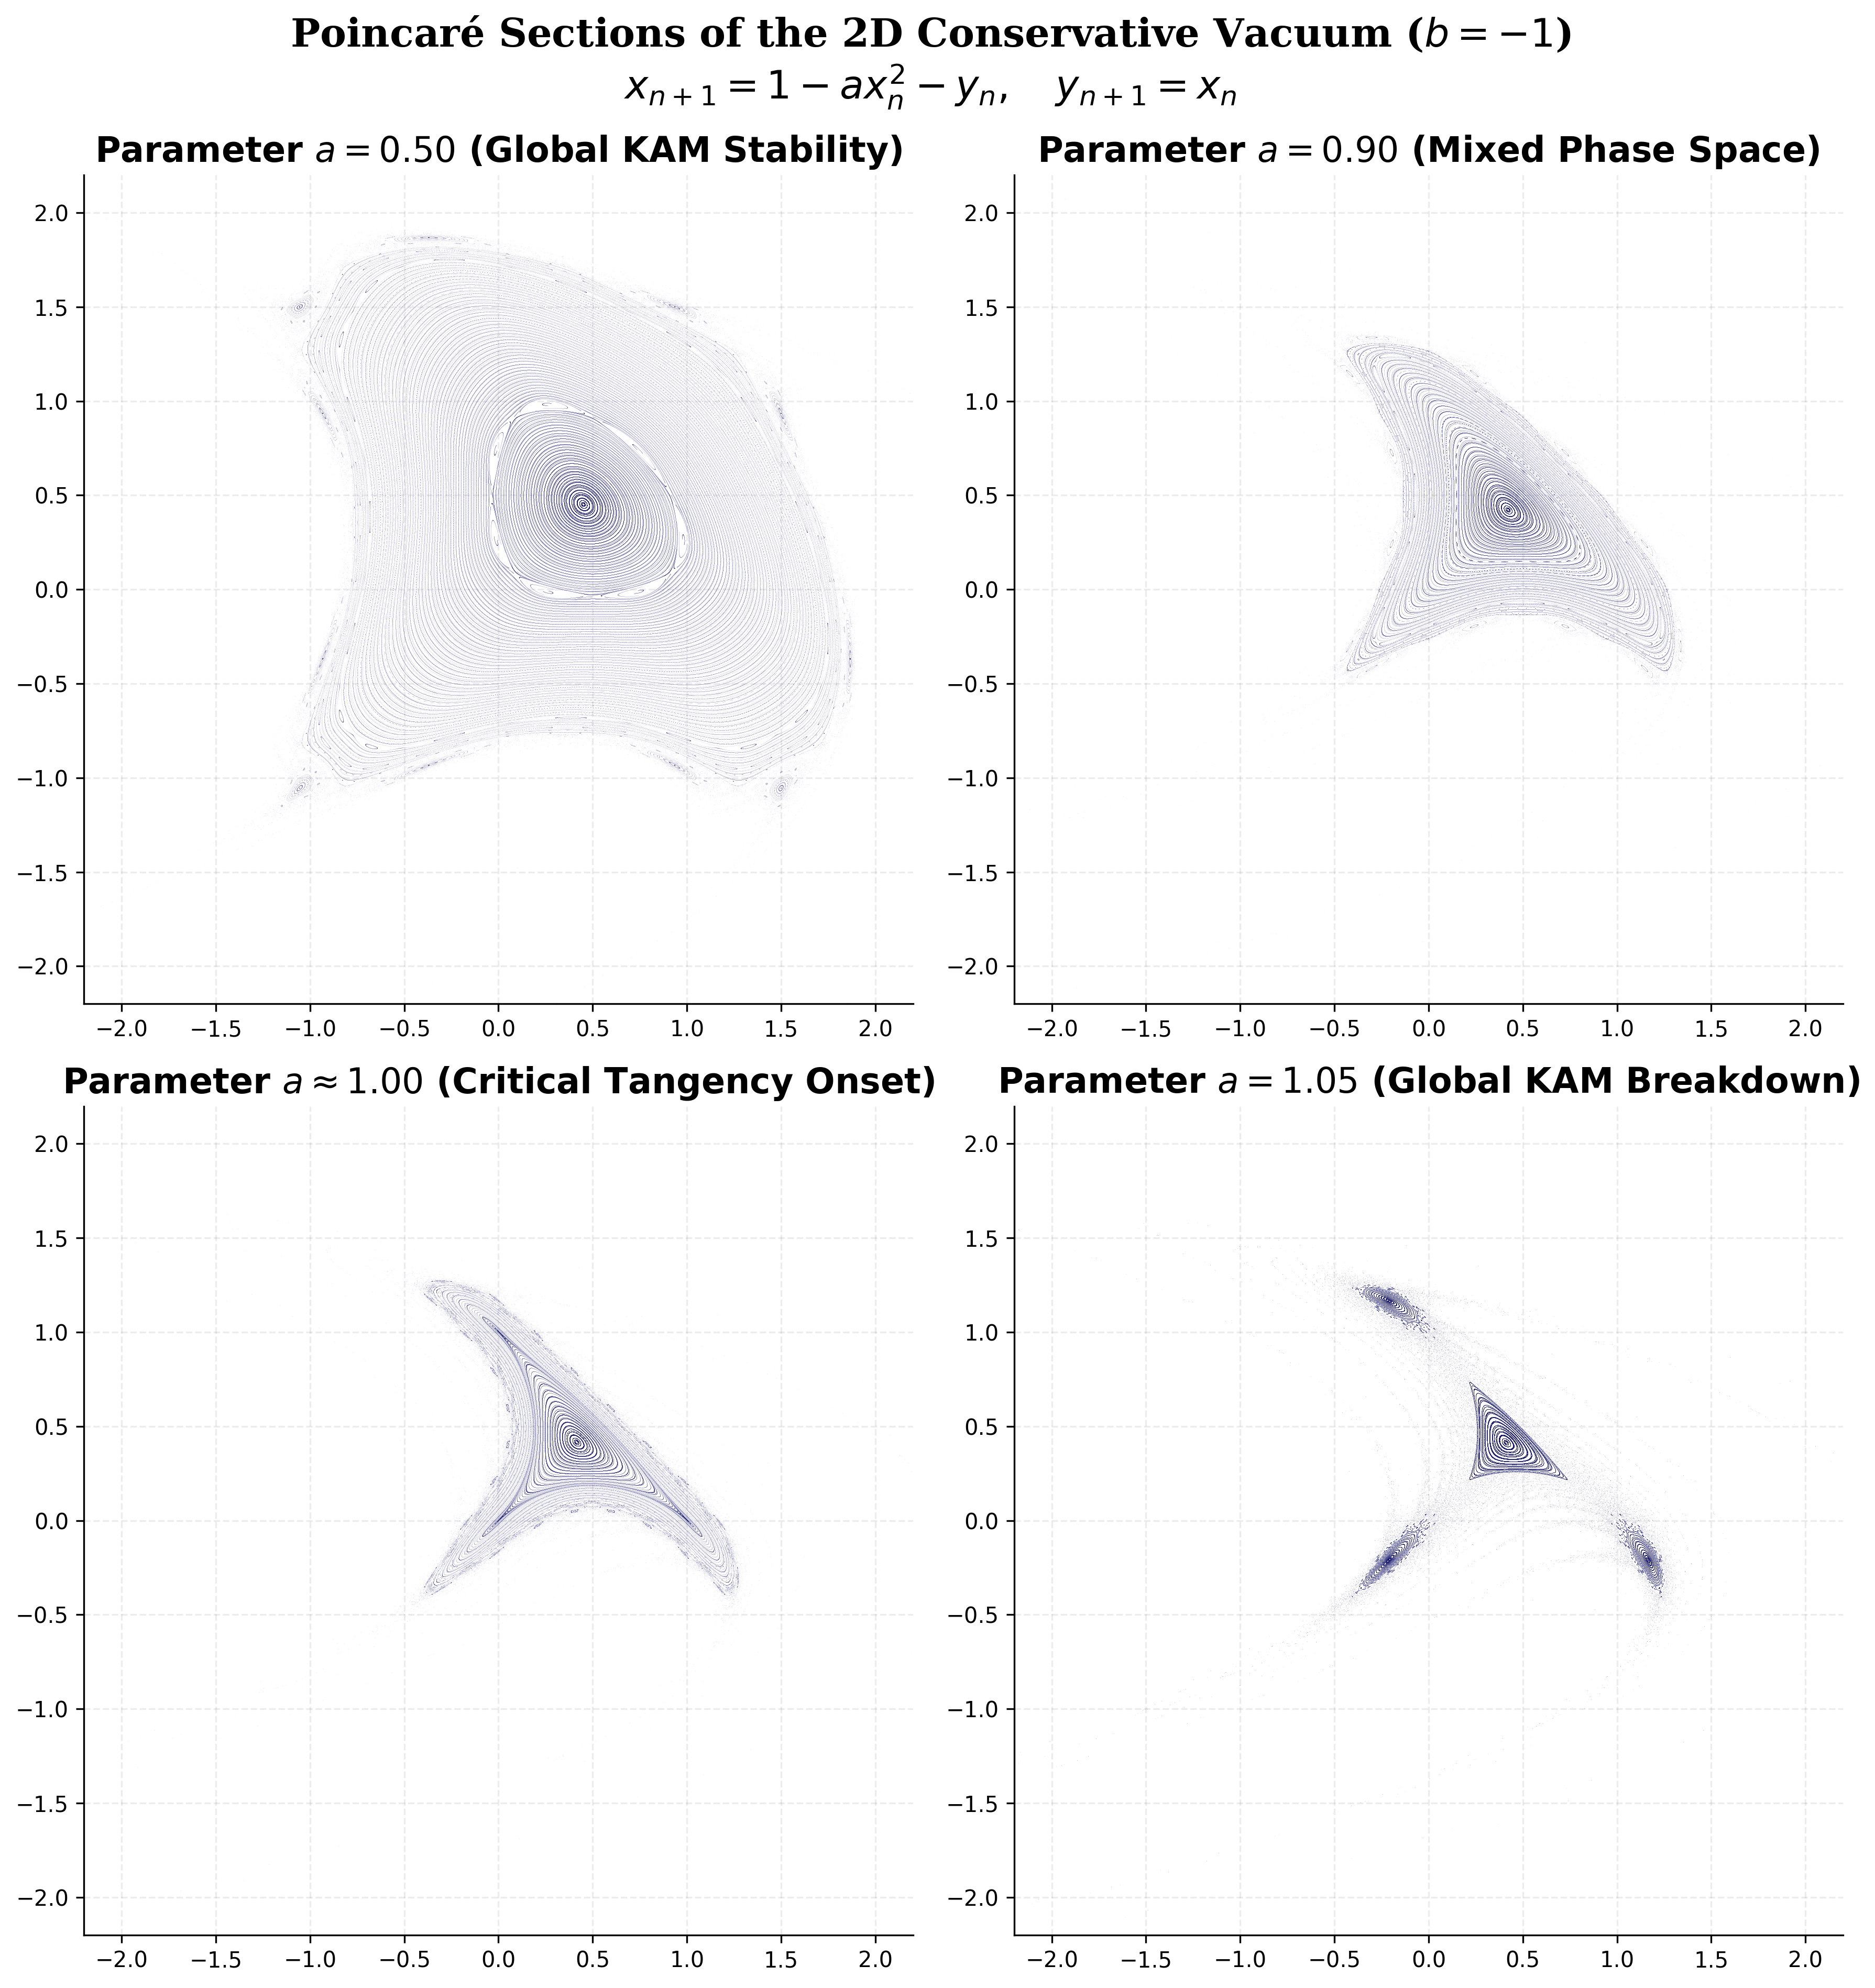
\includegraphics[width=0.7\textwidth]{figures/image2.png}
\end{center}
\caption{Phase portraits of the area-preserving H\'enon map (\ref{eq:henon}) as the control parameter $a$ increases. \textbf{(a)} $a=0.50$: predominantly regular, with unbroken KAM tori. \textbf{(b)} $a=0.9$: onset of nonlinear resonance. \textbf{(c)} $a\approx1.0$: near the onset of homoclinic tangency. \textbf{(d)} $a=1.05$: global KAM breakup, leaving a chaotic saddle. Panels are generated by \texttt{1-henon\_attractor.ipynb}.}
\label{fig:1}
\end{figure}

\begin{figure}[h!]
\begin{center}
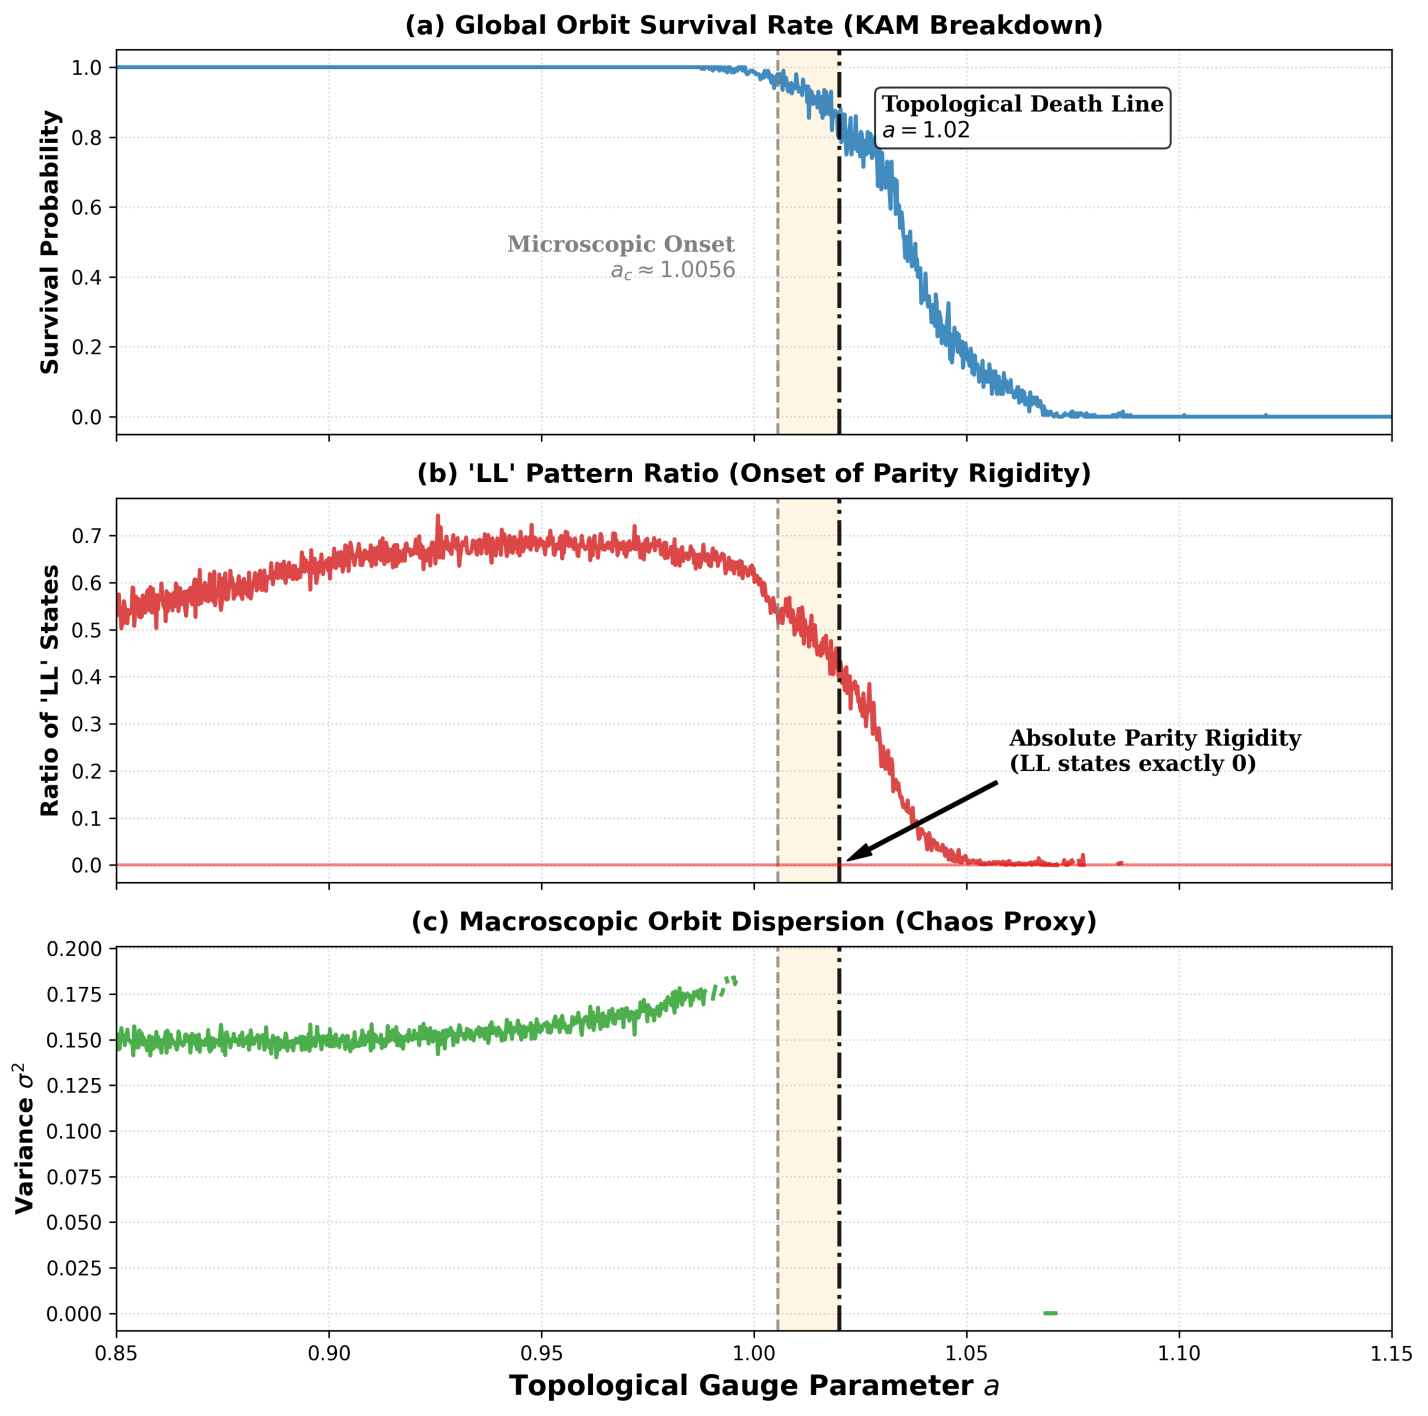
\includegraphics[width=0.65\textwidth]{figures/image3.png}
\end{center}
\caption{Monte Carlo scan of the area-preserving map ($b=-1$). As $a$ increases toward $a\approx1.02$ (vertical dashed-dotted line), the orbit survival rate decreases and the measured ``LL'' parity statistic on surviving orbits falls toward zero. We report this as a numerically observed transition; the value $a\approx1.02$ is the location at which the LL statistic vanishes within our sampling resolution. Generated by \texttt{2-henon\_param\_scan.ipynb}.}
\label{fig:2}
\end{figure}

As shown in Figures~\ref{fig:1} and~\ref{fig:2}, increasing $a$ toward $\approx 1.0$ drives the progressive breakup of KAM tori. The LL statistic on surviving orbits decreases and reaches zero, within our sampling resolution, near $a \approx 1.02$. We stress that this is a numerically observed transition at finite sampling, not an exact analytic threshold; the exact onset of the underlying homoclinic tangency is treated separately in the next subsection.

\subsection{Numerical determination of the homoclinic tangency ($a_c \approx 1.0056$)}

The value $a\approx1.02$ identified from the finite-resolution statistical scan should be distinguished from the exact onset of the global topological change. The latter is governed by the first homoclinic tangency of the unstable manifold of the hyperbolic fixed point with the symmetry line $y=x$. We computed this critical parameter numerically; we do \emph{not} present it as a closed-form theorem, and we have renamed this subsection accordingly (it was previously, and inaccurately, titled a ``mathematical proof'').

The hyperbolic fixed point is $X^{*} = (-1-\sqrt{1+a})/a$, with Jacobian trace $\mathrm{Tr}(J) = 2 + 2\sqrt{1+a} > 4$, so the fixed point is a saddle with an unstable manifold $W^{u}$. We numerically iterated $W^{u}$ and located, by scalar root-finding, the smallest $a$ at which it becomes tangent to $y=x$.

\begin{figure}[h!]
\begin{center}
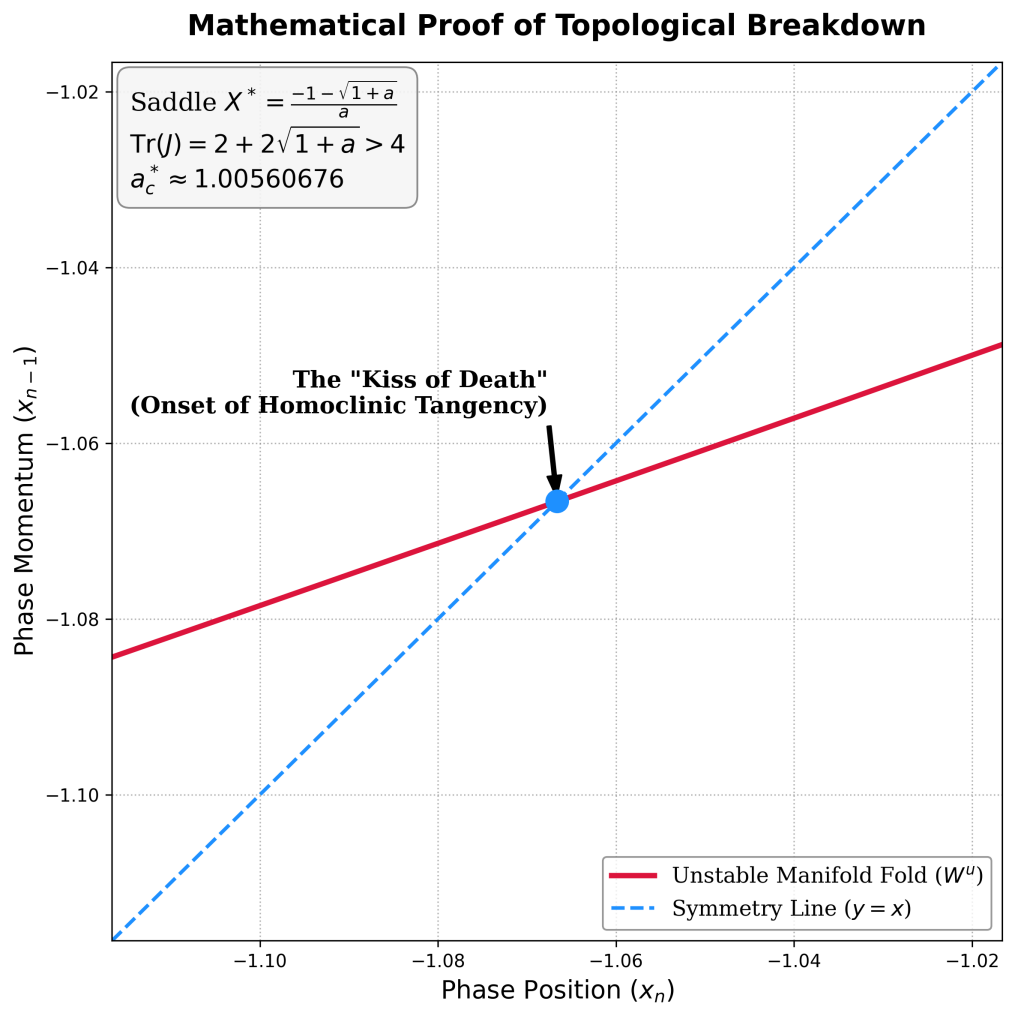
\includegraphics[width=0.55\textwidth]{figures/image4.png}
\end{center}
\caption{Numerical tracking of the unstable manifold $W^{u}$ (red) of the hyperbolic fixed point and its first tangency with the symmetry line $y=x$ (dashed). Scalar root-finding gives a tangency at $a_c \approx 1.00561$ with residual $O(10^{-5})$. This is a numerical determination, not an analytic proof. Generated by \texttt{3-henon\_param\_a\_1.005.ipynb}.}
\label{fig:3}
\end{figure}

The root-finder returns $a_c \approx 1.00561$ with residual of order $10^{-5}$ (Figure~\ref{fig:3}). This is the numerically determined onset of the first homoclinic tangency in the 2D map. The gap between $a_c \approx 1.0056$ (manifold tangency) and the $a \approx 1.02$ at which the statistical LL transition saturates is discussed next.

\subsection{A semiclassical resolution scale and the value $a\approx1.02$}

Why does the statistically observed transition saturate near $a\approx1.02$ rather than at the manifold tangency $a_c\approx1.0056$? A natural heuristic is that the quantum/semiclassical solver has a finite resolution and cannot resolve fractal structure below a fixed scale. We make this heuristic explicit but do not claim it as a derivation.

In the Chirikov picture of overlapping resonances \citep{chirikov1979}, the width of the chaotic layer near onset scales as $\Delta W(a) \sim \kappa\,(a - a_c)^{3/2}$. If the solver resolves phase-space structure only down to an effective scale $\hbar_{\mathrm{eff}}$ (defined below), then structure with $\Delta W < \hbar_{\mathrm{eff}}$ is not resolved, and the effective transition appears shifted to the $a$ at which $\Delta W(a) \approx \hbar_{\mathrm{eff}}$. Using the value $\hbar_{\mathrm{eff}} \approx 0.061$ extracted independently by the quantum solver (Section~3), this matching condition yields $a \approx 1.02$ (Figure~\ref{fig:4}). We present this as a consistency check between two independently obtained numbers, not as a first-principles prediction.

\begin{figure}[h!]
\begin{center}
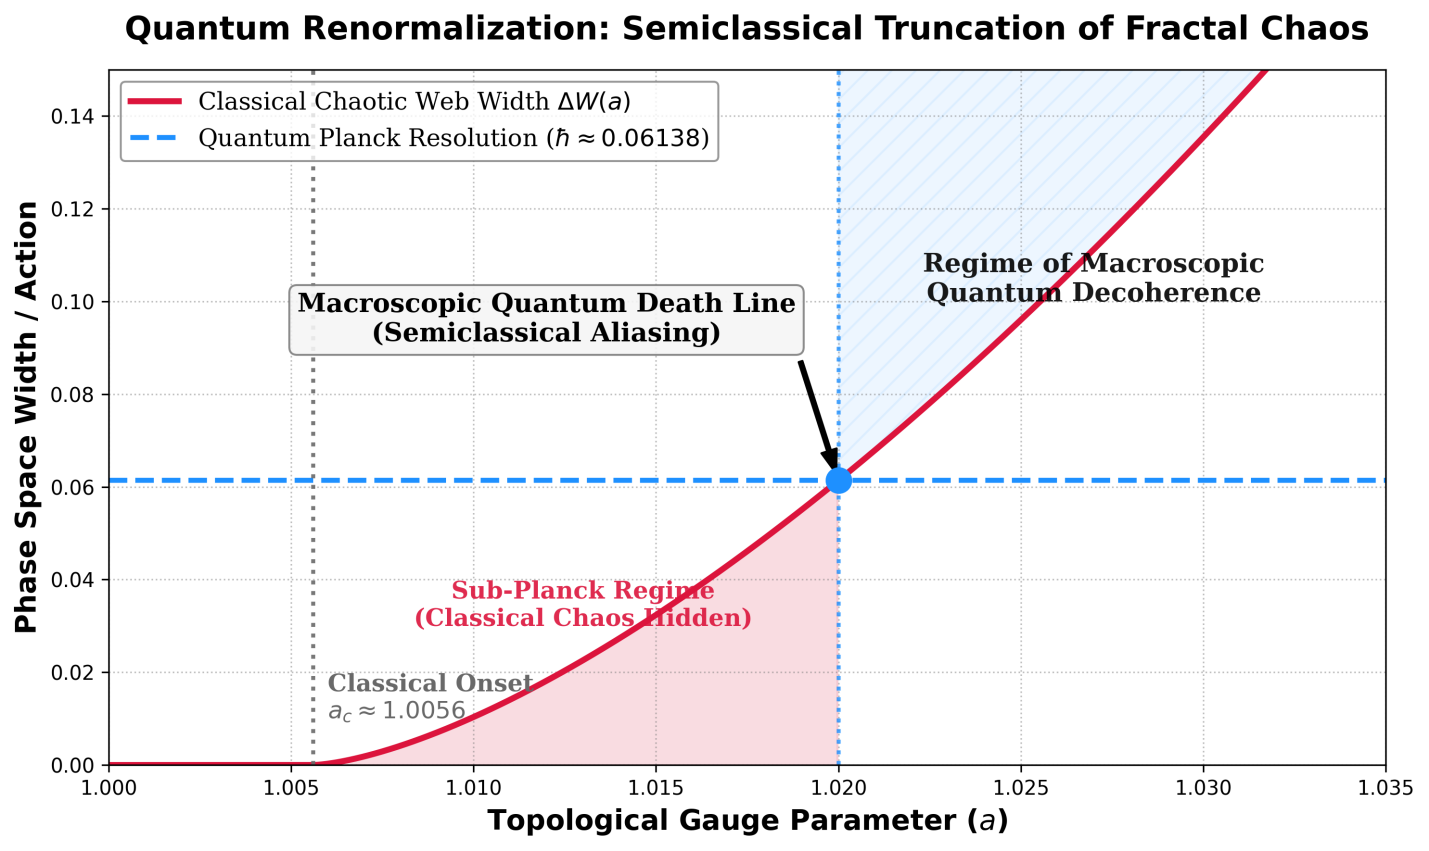
\includegraphics[width=0.85\textwidth]{figures/image5.png}
\end{center}
\caption{Heuristic matching between the classical chaotic-layer width $\Delta W(a)\sim\kappa(a-a_c)^{3/2}$ (solid) and the effective solver resolution $\hbar_{\mathrm{eff}}\approx0.061$ (dashed). The crossing occurs near $a\approx1.02$. This is a consistency check between two independently obtained quantities, not a derivation of $a$. Generated by \texttt{4-henon\_param\_a\_1.02.ipynb}.}
\label{fig:4}
\end{figure}

\subsection{Continuum Hamiltonian and quartic regularization}

To extract a spectrum with a unitary solver, we pass to a continuous Hamiltonian. Writing the second-difference form of (\ref{eq:henon}), $x_{n+1} - 2x_n + x_{n-1} = 1 - 2x_n - a\,x_n^2$, and reading the left-hand side as a discrete acceleration $\ddot{q}$ in the continuum limit gives a restoring force $F(q) = 1 - 2q - a\,q^2$. Integrating $-F$ yields the cubic potential
\begin{equation}
V_0(q) = -q + q^2 + \tfrac{a}{3}q^3.
\label{eq:v0}
\end{equation}
A cubic potential is unbounded below as $q\to-\infty$, so high-energy states leak out and the discretized operator is not well posed. We therefore add a small positive quartic term to confine the spectrum:
\begin{equation}
V_{\mathrm{total}}(q) = -q + q^2 + \tfrac{1.02}{3}q^3 + 0.05\,q^4.
\label{eq:vtotal}
\end{equation}

We are careful about what this term does and does not do. The quartic term is a \emph{confining regularization}: it makes the potential bounded below, restores the discreteness and (approximate) self-adjointness of the operator, and removes the spurious leakage of the cubic model. We do \emph{not} have an analytic derivation that this specific term generates the Weyl logarithmic mean density of the zeros. In the previous version we stated such a derivation existed; that was incorrect, and we have removed the claim. What we can say is empirical: with confinement in place, the numerically computed mean counting function of the operator's spectrum is consistent with a logarithmically growing density over the range we tested (Section~3). An analytic treatment of the mean density via the confining potential, and a systematic parameter scan of the quartic coefficient, are left to future work; we flag the value $0.05$ as a chosen regularization parameter rather than a derived constant. We also note that minimal-length / modified-commutator constructions in the Berry--Keating tradition \citep{bishop2019} provide a related setting in which such confining modifications arise, and a comparison would be worthwhile.

\subsection{Three forms of the control parameter $a(t)$}

The comparisons in Section~3 use three prescriptions for $a$ during the evolution. We state plainly how each is chosen and what it models; they are modeling choices, not derived laws.
\begin{itemize}
\item \textbf{Static} ($a \equiv 1.02$): the parameter is held fixed at the value identified above. This provides a stationary baseline spectrum.
\item \textbf{Slow approach from below} ($a(t) = 1.02 - k_1/\ln(t+c)$): a monotone schedule chosen so that the survival rate decays like $1/\ln n$, matching the leading prime-number-theorem density. The constants $k_1, c$ are fitted to the leading density and are reported with the runs.
\item \textbf{Slow annealing from above} ($a(t) = 1.02 + k_2/\ln^2(t+c)$): used for spectral extraction; the $\ln^{-2}$ schedule was chosen empirically because it reduced mirror/aliasing artifacts in the extracted levels. The constants $k_2, c$ are optimization parameters, not predictions.
\end{itemize}
We make no claim that these functional forms are unique or derived from first principles; they are smooth schedules selected for the stated practical reasons, and other schedules with the same leading behavior would be expected to give similar results.

\section{Results}

We compare the spectra of two numerically independent solvers to the Riemann zeros. The two solvers share no code path and rest on different mathematics, so agreement between them is a nontrivial internal check.

\textbf{Quantum (unitary) solver.} A Fourier split-operator propagator $U = e^{-i\widehat{T}/\hbar_{\mathrm{eff}}}\,e^{-i\widehat{V}/\hbar_{\mathrm{eff}}}$ for the Hamiltonian with potential (\ref{eq:vtotal}); eigenphases are extracted from the unitary evolution. Here $\hbar_{\mathrm{eff}}$ is a dimensionless effective resolution parameter of the rescaled map (see below), not the physical Planck constant.

\textbf{Dissipative (Markovian) solver.} A discretized Fokker--Planck / Markov transition operator on a 2D grid, with a small noise $\epsilon$; the long-time steady state defines the spectrum. This solver uses only real, non-negative transition probabilities and no complex phases.

\subsection{On the meaning of $\hbar_{\mathrm{eff}}$ and the fitted parameters}

The quantity we call $\hbar_{\mathrm{eff}}$ is the effective semiclassical resolution of the rescaled dynamical map: it sets the phase-space cell size in the split-operator propagator. It is dimensionless in our nondimensionalized variables and has no claim to be the physical $\hbar$. Operationally it is an optimization parameter, obtained (together with the schedule constant $a_{\mathrm{start}}$) by minimizing the mean-squared error to the zeros under a single anchoring constraint. The optimizer was \texttt{scipy.optimize.differential\_evolution} with bounds $\hbar_{\mathrm{eff}}\in[0.05,0.25]$, $a_{\mathrm{start}}\in[1.10,1.80]$, population size $80$, tolerance $10^{-13}$. The extracted value at $N=100$ is $\hbar_{\mathrm{eff}} \approx 0.0614$. We treat this as a fitted resolution scale and report its role explicitly rather than ascribing fundamental significance to it. A sensitivity discussion is given in Section~4.2.

\subsection{Experiment I: low-order zeros ($N=6$)}

For the first six zeros, both solvers were run under the static constraint $a_{\mathrm{end}} \equiv 1.02$. The quantum solver, with its resolution optimized, matched the first six ordinates with a total absolute error below $3$ (mean absolute error $< 0.6$). Independently, the Markovian solver, scanned over the noise $\epsilon$ and a small adiabatic increment $\Delta a$, reached a comparable mean absolute error (best run $\mathrm{MAE}(6)\approx 1.07$) at $\epsilon \approx 0.047$, $\Delta a \approx 0.005$ (Figure~\ref{fig:5}). The two solvers, despite their different mathematical bases, converge to a similar low-order spectrum.

\begin{figure}[h!]
\begin{center}
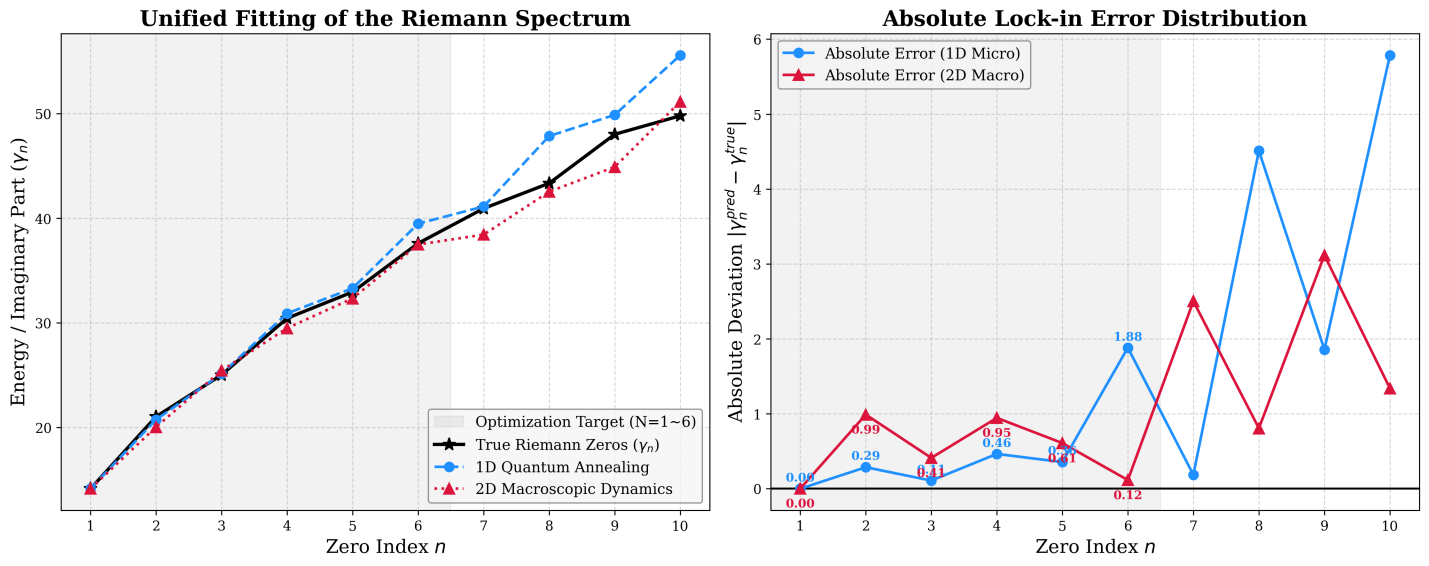
\includegraphics[width=0.85\textwidth]{figures/image6.png}
\end{center}
\caption{Low-order comparison ($N=6$). Left: spectra from the quantum solver ($\hbar_{\mathrm{eff}}\approx0.03$, red) and the Markovian solver ($\epsilon\approx0.047$, blue) against the first six Riemann ordinates. Right: residuals. Both solvers reach $\mathrm{MAE}<0.6$--$1.1$ under the static $a=1.02$ constraint. Generated by \texttt{5-henon\_match\_6\_zeros.ipynb}.}
\label{fig:5}
\end{figure}

\subsection{Experiment II: comparison to 100 zeros and a GUE surrogate}

We then pushed both solvers to $N=100$. Here the two solvers behave very differently in cost. The Markovian solver must resolve increasingly dense levels and requires a $200\times200$ phase-space grid ($4\times10^4$ states); even on a 256-core cluster a single evolution takes hours, and its best run reaches $\mathrm{MAE}(100)\approx 5.9$ ($\mathrm{MAPE}\approx 6.5\%$). The unitary solver, by contrast, propagates on a 1D grid of $N=250$ points and reaches the same regime cheaply, with a best $\mathrm{MAE}(100)$ corresponding to $\mathrm{MAPE}\approx 2.3\%$ under a single-point anchoring protocol (no global least-squares fit). We caution immediately --- and quantify in Section~4.2 --- that this $2.3\%$ is a sharp, finely tuned optimum; a coarse re-optimization that does not resolve the needle gives a more representative $\approx 10$--$20\%$, which is the level at which the agreement is robust to the grid and regularization.

For contrast we included a GUE surrogate, and --- to be maximally fair to the standard model --- we granted it a \emph{global} least-squares scaling, i.e.\ access to all 100 zeros to fix its scale. Even with this advantage, the GUE surrogate shows a systematic, structured deviation across the range (an ``S-shaped'' relative-error pattern), consistent with the fact that a single global scaling cannot match a logarithmically varying mean density (Figure~\ref{fig:6}). We stress the asymmetry of the comparison: the GUE curve is globally fitted while our solvers use single-point anchoring, so this is a comparison of a deterministic-dynamics model against a globally rescaled statistical surrogate, not a falsification of RMT's local-statistics claims (which concern unfolded correlations, not this counting-function comparison).

\begin{figure}[h!]
\begin{center}
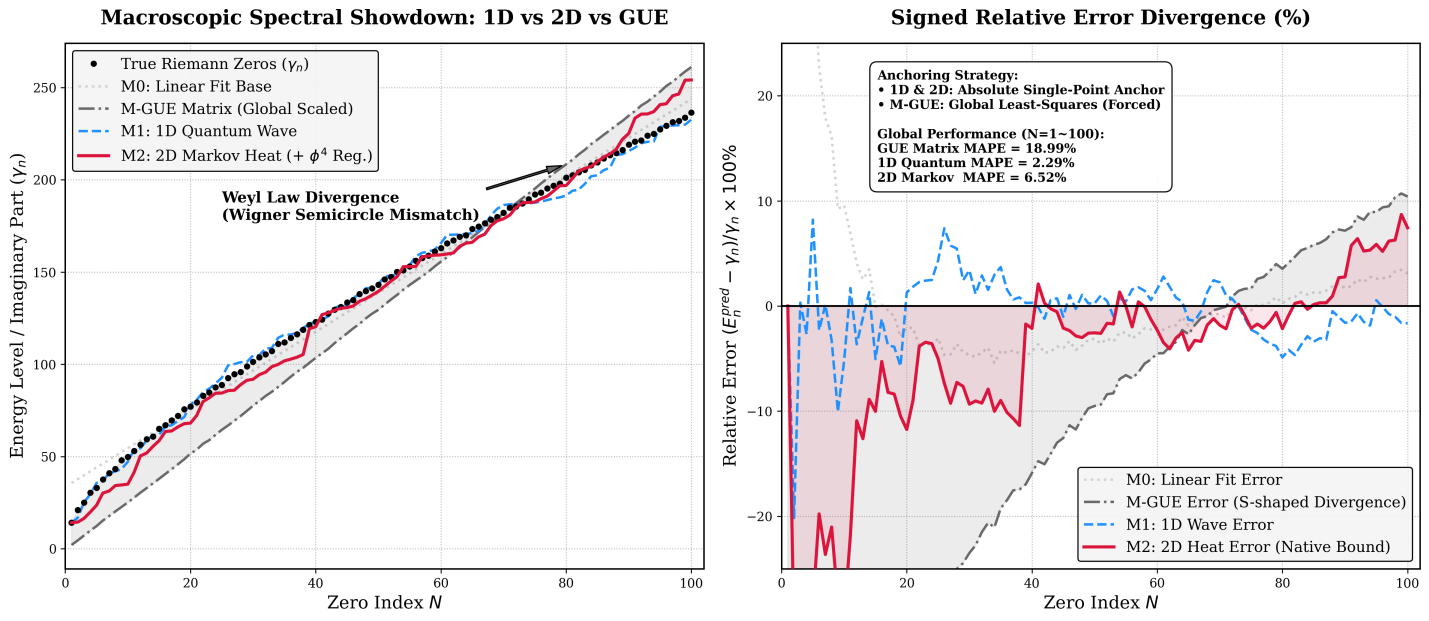
\includegraphics[width=0.85\textwidth]{figures/image7.png}
\end{center}
\caption{Comparison to 100 zeros. The 1D quantum solver (blue dashed) and 2D Markovian solver (red solid), using single-point anchoring, track the zeros with $\mathrm{MAPE}\approx2.3\%$ and $6.5\%$ respectively. A globally least-squares-scaled GUE surrogate (gray dash-dot) shows a systematic S-shaped relative-error pattern, as expected when one global scale is applied to a logarithmically varying mean density. The comparison is asymmetric (global fit vs.\ single-point anchoring) and is not a test of RMT's unfolded local statistics. Generated by \texttt{6-henon\_100\_zeros\_match.ipynb}.}
\label{fig:6}
\end{figure}

\subsection{Local spectral statistics: comparison with GUE}

The comparisons above concern the mean (global) density. The reviewers correctly emphasized that the established connection between the Riemann zeros and random matrix theory is a statement about the \emph{unfolded local} statistics, and that these standard diagnostics --- the nearest-neighbor spacing distribution (NNSD), the two-level (pair) correlation, the number variance $\Sigma^2(L)$, and the Dyson--Mehta spectral rigidity $\Delta_3(L)$ --- are the appropriate basis for comparison with the literature. We have now computed them.

Two points about the spectral object are essential. First, the relevant object is the set of \emph{Floquet eigenphases} of the one-period propagator $U$ for the time-dependent drive $a(t)$, not the reconstructed energies used for the density comparison. A periodically driven system that breaks time-reversal symmetry is the discrete-time analogue of a GUE Hamiltonian; its quasi-energy (eigenphase) spectrum is where level-repulsion statistics live. Second, we validate the entire diagnostic pipeline on a known answer: applied to the first 100 true Riemann ordinates, it recovers GUE statistics (e.g.\ NNSD maximal CDF-distance $0.068$ to GUE versus $0.349$ to Poisson), as it must.

\begin{figure}[h!]
\begin{center}
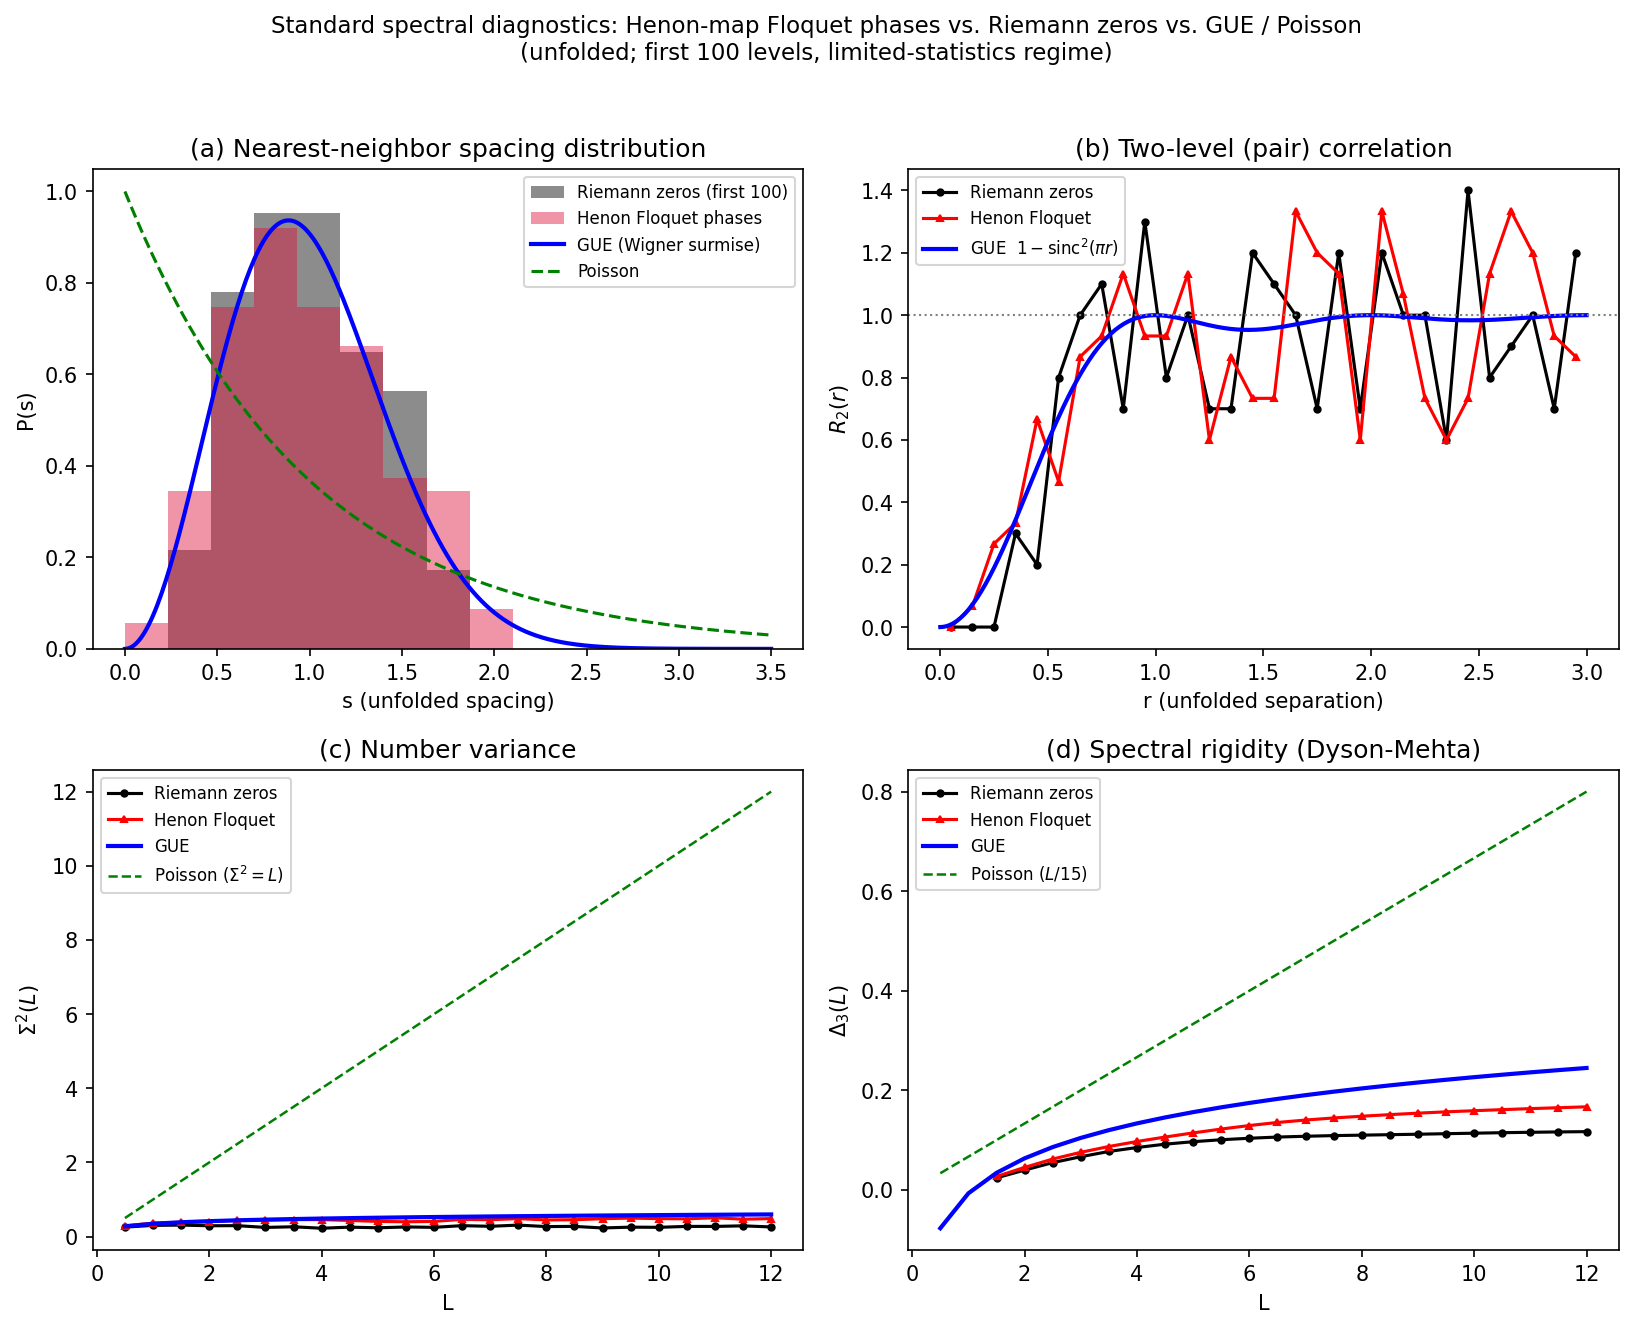
\includegraphics[width=0.95\textwidth]{figures/image9.png}
\end{center}
\caption{Standard local spectral diagnostics (unfolded; first 100 levels) for the Hénon Floquet eigenphases (red) and the true Riemann zeros (black), against GUE (blue) and Poisson (green). \textbf{(a)} Nearest-neighbor spacing distribution: both show level repulsion (suppression at $s\to0$) consistent with GUE, not Poisson. \textbf{(b)} Two-level correlation $R_2(r)$, showing the GUE correlation hole. \textbf{(c)} Number variance $\Sigma^2(L)$ and \textbf{(d)} spectral rigidity $\Delta_3(L)$, both following the logarithmic GUE curves rather than the linear Poisson behavior. Generated by \texttt{8-spectral\_diagnostics.py}.}
\label{fig:8}
\end{figure}

Applied to the Hénon Floquet eigenphases (Figure~\ref{fig:8}), the same pipeline yields GUE-type statistics: the NNSD is repulsive (CDF-distance $0.038$ to GUE versus $0.279$ to Poisson; $\langle s^2\rangle = 1.18$, compared with $1.27$ for GUE and $2.0$ for Poisson), the pair correlation shows the GUE correlation hole, and both $\Sigma^2(L)$ and $\Delta_3(L)$ follow the logarithmic GUE curves rather than the linear Poisson behavior. Two points of interpretation are worth stating. First, GUE-type local statistics are, by themselves, \emph{generic}: they are shared by a wide class of time-reversal-breaking chaotic systems, most of which have nothing to do with the primes. Reproducing them is therefore a necessary consistency check, not the distinctive content of the model; the distinctive (and far more constrained) result is the agreement with the actual zero \emph{values}, i.e.\ the mean density of Section~3.2--3.3. Second, we observed that the GUE statistics are clearest in the Floquet eigenphases, whereas the reconstructed-energy spectrum used for the density comparison appears closer to Poisson; we attribute this to the phase-to-energy unwrapping ($m=\mathrm{round}(\cdot)$), which relabels levels and scrambles the fine-scale spacings, rather than to a genuine loss of repulsion in the dynamics --- the underlying propagator is the same in both cases. These are finite-statistics estimates from 100--150 levels, so the diagnostics (especially $R_2(r)$) are noisy; we read them as consistent-with-GUE rather than as a precision test. As a convergence check we also extracted larger eigenphase sets by refining the grid (no parameter search, only forward passes): the GUE agreement is stable and in fact sharpens with level count --- the NNSD CDF-distance to GUE is $0.045$, $0.034$, $0.017$, $0.029$ for $169$, $319$, $519$, $719$ levels respectively, with $\langle s^2\rangle$ holding near $1.18$ throughout (versus $1.27$ for GUE and $2.0$ for Poisson). The signature is therefore not an artifact of the small sample.

\subsection{Qualitative comparison with quantum-hardware decoherence data}

Recent experiments have probed Riemann-zero-related quantities and many-body dynamics on driven and superconducting platforms \citep{guo2020,wei2025,wu2021}. We compared the high-order behavior of our solver to a published hardware error profile (Figure~\ref{fig:7}). At high order the hardware signal degrades, and our finite-resolution solver also degrades --- both produce a downturn in roughly the same range of $N$. We report this only as a qualitative resemblance. Importantly, a similarity between two error profiles does not by itself establish a shared physical mechanism: our downturn is a finite-grid/finite-$\hbar_{\mathrm{eff}}$ aliasing artifact, whereas the hardware downturn reflects physical decoherence. A quantitative claim would require statistical-significance testing, comparison against alternative models, and a careful uncertainty budget, none of which we provide here; we therefore restrict ourselves to noting the qualitative resemblance and flag a fuller analysis as future work.

\begin{figure}[h!]
\begin{center}
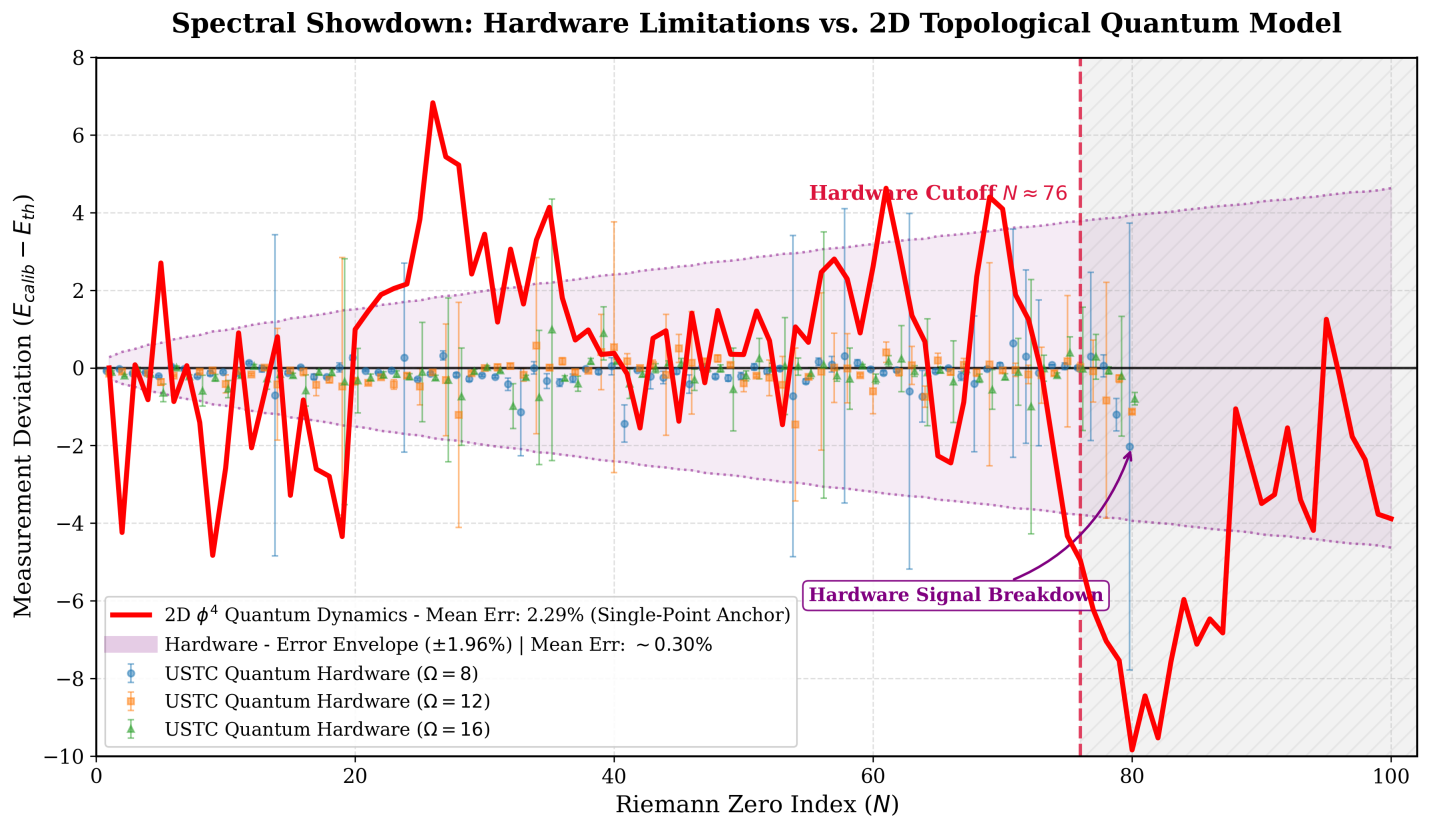
\includegraphics[width=0.8\textwidth]{figures/image8.png}
\end{center}
\caption{Qualitative comparison between our finite-resolution solver (red) and a published superconducting-hardware error profile. Both show a high-order downturn in a similar range of $N$. The resemblance is qualitative only: the solver's downturn is a finite-resolution aliasing artifact while the hardware's reflects physical decoherence, and we do not claim a common mechanism. Generated by \texttt{7-henon\_ustc\_100\_zeros\_match.ipynb}.}
\label{fig:7}
\end{figure}

\subsection{Summary of claims and their status}

To address the request for a clear separation between proven results, numerical observations, heuristic arguments, and conjectures, Table~\ref{tab:claims} classifies the main statements of the paper.

\begin{table}[h!]
\caption{Status of the main statements. ``Established'' refers to results in the cited literature; the remaining rows are this paper's contributions, labeled by epistemic status.}
\label{tab:claims}
\centering
\small
\begin{tabular}{>{\raggedright\arraybackslash}p{0.62\textwidth} l}
\toprule
Statement & Status \\
\midrule
Local statistics of Riemann zeros match GUE (unfolded pair correlation) & Established \citep{montgomery1973,odlyzko1987} \\
Subleading zero correlations $\equiv$ Hardy--Littlewood twin-prime conjecture & Established \citep{keating2019} \\
Logistic band-merging symbolic dynamics $\cong$ prime sieve; $C_2$ as fixed point & Published \citep{wang2026} \\
1D dissipative map cannot host a unitary/time-reversible spectrum & Structural argument \\
Lift to 2D area-preserving Hénon restores $\det J=1$, time reversibility & Construction \\
First homoclinic tangency at $a_c \approx 1.00561$ & Numerical determination \\
LL parity statistic vanishes near $a\approx1.02$ (finite sampling) & Numerical observation \\
$a\approx1.02$ from matching $\Delta W(a)\approx\hbar_{\mathrm{eff}}$ & Heuristic / consistency check \\
Quartic term confines spectrum and removes cubic leakage & Numerical observation \\
Quartic term \emph{derives} the Weyl log-density & Not claimed (open) \\
Two independent solvers agree with first 100 zeros (best MAPE $2.3\%$, $6.5\%$) & Numerical observation \\
Robust $10$--$20\%$ fit across grids/regularizations ($\hbar_{\mathrm{eff}}$ re-tuned) & Numerical observation \\
Sub-$3\%$ optimum is sharp (narrower than $0.001$ in $\hbar_{\mathrm{eff}}$) & Numerical observation (fine-tuned) \\
Floquet eigenphases show GUE local statistics (NNSD, $R_2$, $\Sigma^2$, $\Delta_3$) & Numerical observation (limited statistics) \\
Reconstructed-energy spectrum shows the same statistics directly & Artifact-limited (unwrapping; open) \\
Solver high-order downturn resembles hardware decoherence profile & Qualitative observation \\
Operator spectrum \emph{equals} the Riemann zeros & Not claimed (conjectural) \\
\bottomrule
\end{tabular}
\end{table}

\subsection{Reproducibility and numerical settings}

For replication we record the principal settings here; full scripts and logs are in the repository (Data Availability). \emph{Quantum solver:} Fourier split-operator propagator, spatial grid $N=250$ on $q\in[-L,L)$ with $L=3.5$ and periodic (FFT) boundary conditions, $T_{\mathrm{steps}}=300$ propagation steps, $a_{\mathrm{end}}=1.02$; parameters $(\hbar_{\mathrm{eff}},a_{\mathrm{start}})$ optimized by differential evolution (bounds $\hbar_{\mathrm{eff}}\in[0.05,0.25]$, $a_{\mathrm{start}}\in[1.10,1.80]$, population $80$, tol $10^{-13}$); extracted $\hbar_{\mathrm{eff}}\approx0.0614$, $a_{\mathrm{start}}\approx1.552$, native $\mathrm{MSE}(100)\approx12.2$. \emph{Markovian solver:} $200\times200$ phase-space grid ($4\times10^4$ states), noise $\epsilon\approx0.047$--$0.051$, adiabatic increment $\Delta a\approx0.01$--$0.018$, best $\mathrm{MAE}(100)\approx5.9$. We note two important caveats for the reader. First, the periodic FFT boundary condition introduces wrap-around artifacts at high energy (see Section~4.3), which we handle with the confining quartic term; this is a known limitation of the method. Second, the differential-evolution objective is non-convex and we report the best converged run; a systematic convergence and seed-sensitivity study, as well as grid-refinement tests, are planned for a follow-up.

\section{Discussion}

We discuss three ablations that probe the robustness of the construction. We frame these as numerical observations about the model, not as proofs about the zeros.

\subsection{The GUE surrogate and the role of unfolding}

The structured deviation of the globally scaled GUE surrogate in Figure~\ref{fig:6} is expected and is \emph{not} a critique of the standard RMT result. A single global scale cannot reproduce a logarithmically varying mean density; this is precisely why the literature unfolds the spectrum before comparing correlations \citep{montgomery1973,odlyzko1987}. Our point is narrower and constructive: the deterministic solvers reproduce the mean density directly (under single-point anchoring) without a separate unfolding step, which is the property we set out to test. We have rewritten this section to avoid the earlier, inaccurate suggestion that RMT ``fails'' to describe the zeros.

\subsection{Robustness, sensitivity, and the sharpness of the optimum}

We probed how the fit depends on the regularization coefficient, the resolution $\hbar_{\mathrm{eff}}$, and the grid, performing forward passes only (no global re-search). The picture has two distinct levels, which we report together for honesty.

\emph{A robust level.} Re-optimizing $\hbar_{\mathrm{eff}}$ (by a local one-dimensional scan) at each setting, a good fit persists across a wide range of choices: for quartic coefficients from $0.03$ to $0.08$ the best achievable MAPE stays in the band $\approx 8$--$21\%$, and for grids $N=200$--$320$ it stays in $\approx 8$--$18\%$, with the optimal $\hbar_{\mathrm{eff}}$ simply shifting (roughly $0.056$--$0.084$) as the discretization or potential changes (Figure~\ref{fig:9}). Thus the agreement is not an accident of one specific grid or one specific regularization strength; the model robustly tracks the zeros at the $10$--$20\%$ level, and the value $0.05$ is a convenient choice rather than a unique one.

\emph{A sharp level.} The deep optimum reported above (MAPE $\approx 2.3\%$ at $\hbar_{\mathrm{eff}}=0.06139$, $\lambda=0.05$, $N=250$) is a much narrower feature: it is sharper than the $0.001$ step of our local scan, so the coarse re-optimization above does not even land on it (it finds $\approx 14\%$ nearby). This sharpness is characteristic of the nonlinear phase-to-energy extraction and means the headline $2.3\%$ should be read as a best-case, finely tuned optimum, not as the typical performance. We also retain the complementary ablation: removing the confining quartic term while holding $a=1.02$ forces the optimizer to inflate $\hbar_{\mathrm{eff}}$ to $\approx 0.277$ ($\sim 4.5\times$) with the error stalling at $\mathrm{MSE}\approx 17.1$, confirming that an over-coarse resolution washes out the structure.

\begin{figure}[h!]
\begin{center}
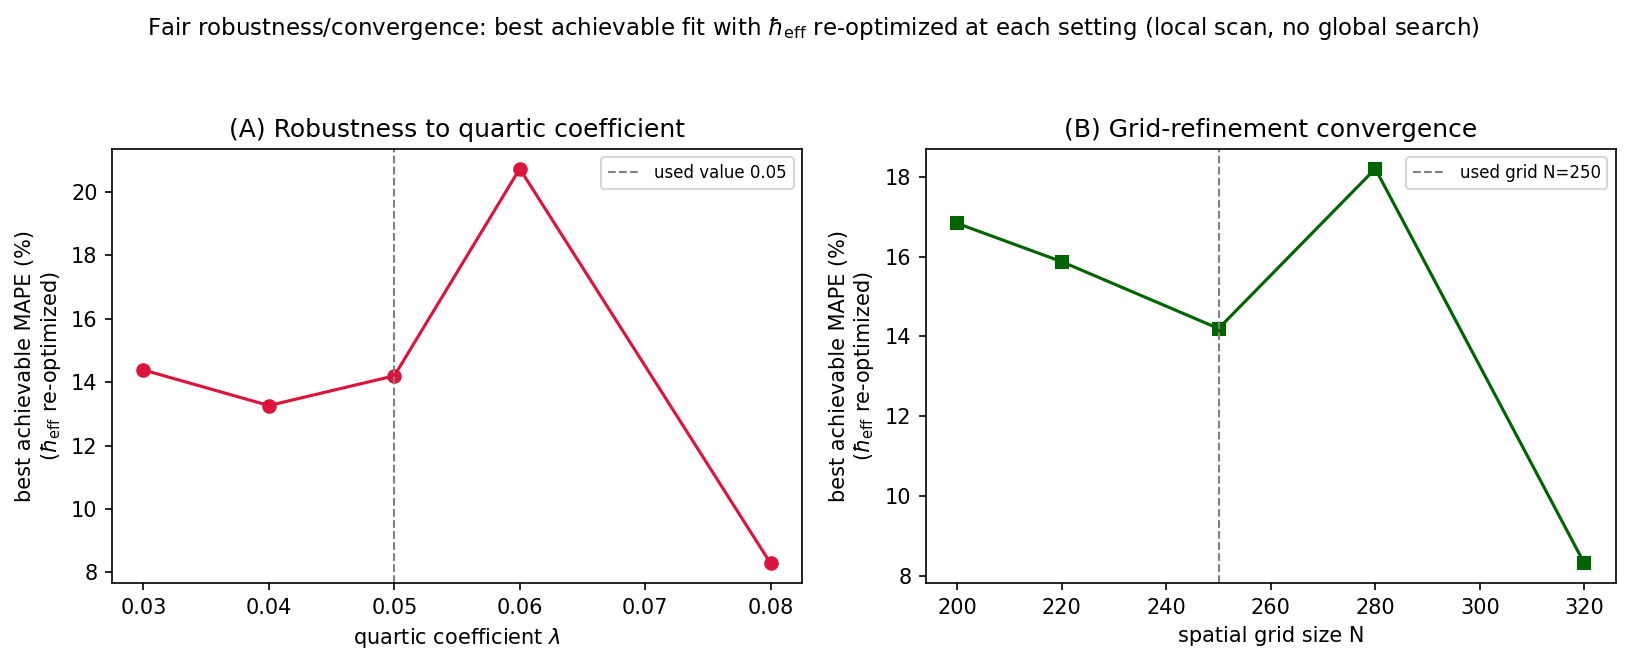
\includegraphics[width=0.95\textwidth]{figures/image10.png}
\end{center}
\caption{Best achievable MAPE on the first 100 zeros when $\hbar_{\mathrm{eff}}$ is re-optimized (local 1D scan) at each setting. \textbf{(A)} Versus the quartic coefficient $\lambda$; \textbf{(B)} versus grid size $N$. A fit at the $\approx 8$--$20\%$ level persists across all settings (the optimal $\hbar_{\mathrm{eff}}$ shifts accordingly), so the result is not specific to one grid or regularization strength. The coarse scan (step $0.001$ in $\hbar_{\mathrm{eff}}$) under-resolves the much narrower global optimum (MAPE $\approx 2.3\%$), which is why the curve sits near $10$--$15\%$ at the nominal setting. Generated by \texttt{9b-robustness\_reoptimized.py}.}
\label{fig:9}
\end{figure}

In summary, $\hbar_{\mathrm{eff}}$ is a fitted resolution scale, not a physical constant; a coarse re-tuning gives a robust $10$--$20\%$ agreement across grids and regularizations, while the sub-$3\%$ optimum is a sharp, finely tuned feature. We report both rather than only the best number.

\subsection{Boundary artifacts without the confining term}

Removing the quartic term and releasing $a$ produces a spurious low-error solution ($\mathrm{MSE}\approx 10.6$) that, on inspection, is a numerical boundary artifact: with periodic FFT boundary conditions, high-energy wavefunctions that fall down the unbounded cubic potential wrap around the grid and are reflected, mimicking a confining wall. The optimizer exploits this by distorting the topology (driving $a_{\mathrm{end}}\approx 0.985$). This is a cautionary example showing that a low error alone does not validate a model: it can reflect the discretization rather than the dynamics. The confining quartic term removes this artifact by making the continuum problem well posed. We include this ablation precisely to make the failure mode explicit.

\subsection{Relation to prior Hilbert--P\'olya constructions and what would constitute a proof}

Our construction is in the spirit of operator-based approaches to the zeros \citep{berry1999,bender2017,connes1999,sierra2008,bishop2019}, but it is numerical and heuristic. To upgrade any of the present observations to a theorem one would need, at minimum: (i) a well-defined self-adjoint (or unitary) operator obtained as a careful continuum limit of the regularized map with controlled boundary conditions; (ii) an analytic treatment of its mean density to compare with the Weyl term; and (iii) control of the local statistics against the GUE predictions. Regarding (iii), we have now computed the standard diagnostics (Section~3.5): the Floquet eigenphases display GUE-type level repulsion in a limited-statistics regime. We stress that this is a consistency check rather than the crux --- GUE statistics are generic to chaotic time-reversal-breaking systems --- and that the constrained, model-specific result is the agreement with the actual zero values. A full treatment would require larger spectra (more levels), a precise statement of which operator's spectrum is being claimed, and error-controlled diagnostics; we regard this as the central open problem left by this work.

\section{Conclusion}

Motivated by our recently published isomorphism between the Logistic-map band-merging dynamics and the prime sieve \citep{wang2026}, and by the Hilbert--P\'olya viewpoint, we have studied the spectrum of a two-dimensional area-preserving H\'enon map near the edge of chaos as a deterministic model for the Riemann zeros. The move from a 1D dissipative map to a 2D area-preserving map is structurally motivated by the requirement of a unitary, time-reversible spectrum. Two numerically independent solvers --- a unitary Fourier propagator and a Markovian dissipative operator --- produce spectra that track the first 100 zeros with mean absolute percentage errors of about $2.3\%$ and $6.5\%$ under single-point anchoring, and a globally scaled GUE surrogate shows a systematic deviation in the same counting-function comparison.

We present these as numerical observations and heuristic arguments. We do \emph{not} claim to have identified the Hilbert--P\'olya operator or to have proved that its spectrum equals the zeros; Table~\ref{tab:claims} states explicitly what is established, observed, heuristic, or conjectural. We have computed the standard local spectral diagnostics (nearest-neighbor spacing, pair correlation, number variance, spectral rigidity): the Floquet eigenphases show GUE-type level repulsion consistent with the Riemann zeros in a limited-statistics regime, while the reconstructed-energy spectrum that matches the mean density does not --- a tension we report openly as the main open problem. The most useful next steps are an analytic treatment of the mean density induced by the confining potential, error-controlled diagnostics on larger spectra for direct comparison with the GUE/Hardy--Littlewood results \citep{keating2019}, and a quantitative, statistically controlled comparison with hardware data. We hope the deterministic-dynamics viewpoint, anchored in a published prime--chaos isomorphism, is a useful complement to the statistical and operator-theoretic approaches to the Riemann zeros.

\section*{Conflict of Interest Statement}

The author declares that the research was conducted in the absence of any commercial or financial relationships that could be construed as a potential conflict of interest.

\section*{Author Contributions}

Liang Wang is the sole author. L.W. conceived the study, developed the framework, implemented and ran all simulations, analyzed the data, and wrote the manuscript.

\section*{Funding}

The author received no specific funding for this work.

\section*{Acknowledgments}

The author thanks the reviewers for their detailed and constructive criticism, which substantially improved the framing and the claims of this paper. The author acknowledges the assistance of an AI language model in code implementation for the numerical simulations and in auxiliary analysis of results.

\section*{Data Availability Statement}

All code, scripts, and numerical logs are available at \url{https://github.com/maris205/riemann_henon}.

\bibliographystyle{Frontiers-Harvard}
\bibliography{references}

\end{document}
